\documentclass[a4paper,12pt]{article}
%\documentclass[a4paper,10pt]{scrartcl}

\usepackage[utf8]{inputenc}
\usepackage{siunitx}
\usepackage{amsmath}
\DeclareSIUnit \voltampere {VA} %apparent power 
\DeclareSIUnit \var {var} %volt-ampere reactive - idle power 
\usepackage{bm}
\usepackage{booktabs}
\usepackage{float}
\usepackage[straight voltages, european resistors, siunitx, RPvoltages]{circuitikz}
\usepackage{hyperref}

\title{ELECTENG209 \\ Team 02:\\ Project Component Values}
\author{Ankush Patel, Daniel Lin, Krithik Lekinwala, Rukin Swedlund}
\date{13/08/2020}

\pdfinfo{%
  /Title    (ELECTENG209 - Team 02: Project Component Values)
  /Author   (Ankush Patel, Daniel Lin, Krithik Lekinwala, Rukin Swedlund)
  /Creator  (Ankush Patel)
  /Keywords (ELECTENG209 TEAM02 Project Component Values)
}

\begin{document}
\maketitle
\newpage

\tableofcontents
\newpage

\section{Introduction}
This document details the circuits and component values we will use to build our project.
The structure and order of the component values and circuits described follow the order of the Labs.

The basic structure of components is as follows:

\begin{center}
 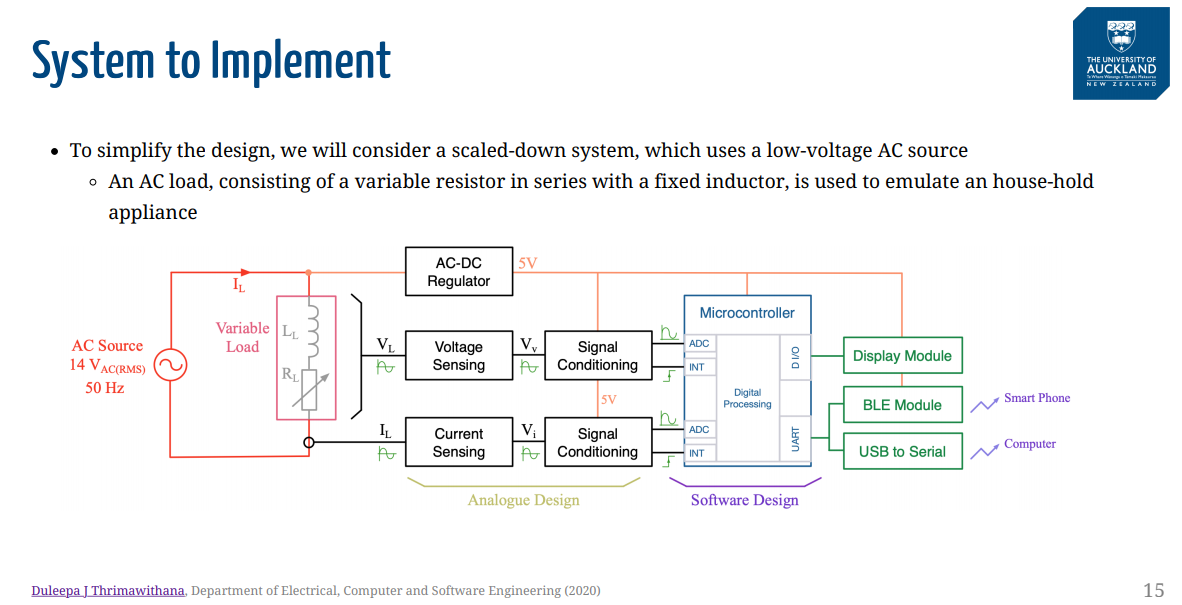
\includegraphics[keepaspectratio=true, scale=0.5]{SysToImpli.png}
\end{center}


All (fixed) component values are based on the \hyperlink{LINK_E12}{The E-12 Series}

\newpage

\section{Voltage \& Current Sensors}

\vspace{5mm}
\begin{circuitikz}[scale=1.5]
 \draw (0, 0) to [sinusoidal voltage source=$V_{ac}$] (0, 8)
	(0, 8) to (6, 8)
	
	% Right Branch (Voltage Sesnor)
	(6, 8) to[R=$R_A$] (6, 4)
	to[R=$R_B$, v=$V_{VS}$] (6, 0)
	to (0, 0)
	
	% Left Branch (Load / Current Sensing)
	(6, 8) to (3, 8) to[L=$L$] (3, 6)
	to[R=$R_L$] (3, 4)
	to[R=$R_S$, v=$V_{IS}$] (3, 0)
	to (0, 0)
	;
\draw[dashed, blue] (2, 8.1) rectangle (4, 4) (3, 8) node[above] {Load};
\draw[dashed, purple] (1.5, 3.5) rectangle (4, 0.5) (2.5, 3.5) node[above] {Current Sensor};
\draw[dashed, orange] (4.5, 7) rectangle (7, 0.5) (8, 7) node[above] {Voltage Sensor};
\end{circuitikz}

\vspace{7mm}

$R_S$ is the Shunt Resistor that we use to measure the current drawn through the load. 

${V_{IS}}$  is the voltage dropped across the shunt resistor ($R_{S}$). 
This drop in voltage is proportional to the current through the shunt resistor 
(and therefore proportional to the current through the load). \medskip

\textbf{The nominated value of $R_S$ is $R_S = 0.56\ \si{\ohm}$}. \medskip


$R_A$ and $R_B$ are the two Voltage Dividers that make up the voltage sensor.
The Voltage sensors output is taken to be the voltage across $R_B$ ($V_{VS}$). \medskip

\textbf{
	The nominated values for $R_A$ and $R_B$ are:
	$R_A = 82\ \si{\kilo\ohm}$ and $R_B = 3.8\ \si{\kilo\ohm}$.
} \medskip


\textbf{The following is a table of values to use for testing the limits of the sensors:}
\medskip

\begin{table}[H]
 \centering
 \renewcommand\arraystretch{2}
 \begin{tabular}{p{4cm} p{4cm} p{2cm}}

 \toprule
 Source $V_{AC}$ & $V_{AC(RMS)}$ & $R_L$ \\
 \toprule
 $7.5\ \si{\voltampere}$ & $12.6\ \si{\volt}$ & $16.65\ \si{\ohm}$ \\
 $7.5\ \si{\voltampere}$ & $15.4\ \si{\volt}$ & $29.00\ \si{\ohm}$ \\
 $2.5\ \si{\voltampere}$ & $15.4\ \si{\volt}$ & $92.82\ \si{\ohm}$ \\
 \bottomrule
 \end{tabular}
\end{table}


\clearpage

\section{Measurement Conditioning}

\vspace{5mm}

\begin{figure}[H]
	\centering
	\begin{circuitikz}[scale=1.5]
	\draw (0, 4) to[short, o-*] (2, 4)
		% Open Circuit Terminals
		(0, 8) to[short, o-*] (2, 8)
		(0.2, 8) to[open, v=$V_{IS}$] (0.2, 4) 

		(6, 6) node[op amp, yscale=-1] (opamp) {}
		(opamp.+) node[left]{$V^+$}
		(opamp.-) node[left]{$V^-$}
		(opamp.out) node[above]{$V_{OUT}$}
		
		% Non-Inverting Terminal
		(2, 8) to[R=$R_1$] (4, 8)
		(4, 8) to[R=$R_2$] (4, 6)
		(3.8, 6) to[short] (4.2, 6)
		(4, 6) node[below]{$2.1\ \si{\volt}$}
		(4, 8) to[short] (4, 8 -| opamp.+)
		to[short] (opamp.+)
		
		% Inverting Terminal
		(2, 4) to[R=$R_1$] (4, 4)
		to[short] (4, 4 -| opamp.-)
		to[short] (opamp.-)
		(4, 4) to[R=$R_2$] (8, 4)

		
		% Negative Feedback
		to[short] (8, 4 |- opamp.out)
		to[short] (opamp.out)	
		;
	\end{circuitikz}
	\caption{Current Signal Conditioning Circuit}
\end{figure}

\vspace{7mm}

The the four resistors of value $R_1$ and $R_2$ control the gain and offset
applied by the Operational Amplifier to the input signal $V_{IS}$.

\medskip

\textbf{The value of $R_1$ and $R_2$ is: $R1 = 39\ \si{\kilo\ohm}$ and $R_2 = 82\ \si{\kilo\ohm}$.}

\begin{figure}[H]
	\centering
	\begin{circuitikz}[scale=1.5]
	\draw (0, 4) to[short, o-*] (2, 4)
		% Open Circuit Terminals
		(0, 8) to[short, o-*] (2, 8)
		(0.2, 8) to[open, v=$V_{VS}$] (0.2, 4) 

		(6, 6) node[op amp, yscale=-1] (opamp) {}
		(opamp.+) node[left]{$V^+$}
		(opamp.-) node[left]{$V^-$}
		(opamp.out) node[above]{$V_{OUT}$}
		
		% Non-Inverting Terminal
		(2, 8) to[R=$R_{1a}$] (4, 8)
		(4, 8) to[R=$R_2$] (4, 6)
		(3.8, 6) to[short] (4.2, 6)
		(4, 6) node[below]{$2.1\ \si{\volt}$}
		(4, 8) to[short] (4, 8 -| opamp.+)
		to[short] (opamp.+)
		
		% Inverting Terminal
		(2, 4) to[R=$R_{1b}$] (4, 4)
		to[short] (4, 4 -| opamp.-)
		to[short] (opamp.-)
		(4, 4) to[R=$R_2$] (8, 4)

		
		% Negative Feedback
		to[short] (8, 4 |- opamp.out)
		to[short] (opamp.out)	
		;
	\end{circuitikz}
	\caption{Voltage Signal Conditioning Circuit}
\end{figure}

\vspace{7mm}

The four resistors of value $R_{1a}$, $R_{1b}$ and $R_2$ control the gain and offset
applied by the Operational Amplifier to the input signal $V_{VS}$.

\medskip

\textbf{The value of $R_{1a}, R_{1b}$ and $R_2$ is: $R_{1a} = 10\ \si{\kilo\ohm}, R_{1b} = 47\ \si{\kilo\ohm}$ and $R_2 = 47\ \si{\kilo\ohm}$}.


\clearpage

\section{Filters}

\vspace{5mm}

\begin{circuitikz}[scale=1.5]
 \draw (0, 4) to[short, o-*] (2, 4)
	% Open Circuit Terminals
	(0, 8) to[short, o-*] (2, 8)
	(0.2, 8) to[open, v=$V_{OpAmp}$] (0.2, 4)
	(2, 8) to[R=$R_f$] (4, 8)
	to[C=$C_f$] (4, 4)
	to[short] (2, 4)
	% Open Circuit Terminals
	(4, 8) to[short, *-o] (6, 8)
	(4, 4) to[short, *-o] (6, 4)
	(6, 8) to[open, v=$V_{filter}$] (6, 4)
	;
\end{circuitikz}

\vspace{7mm}

The Resistor and Capacitor create a filter that has a breakpoint frequency of $100\ \si{\kilo\hertz}$. 

\medskip

\textbf{The value of $R_f$ and $C_f$ is: $R_f = 33\ \si{\kilo\ohm}$ and $C_f = 4.8\ \si{\nano\farad}$}.


\clearpage

\section{The E-12 Series:}
\hypertarget{LINK_E12}{}

\begin{align*}
	1.0\ \si{\ohm} \hspace{4mm} 
	1.2\ \si{\ohm} \hspace{4mm} 
	1.5\ \si{\ohm} \hspace{4mm} 
	1.8\ \si{\ohm} \hspace{4mm} 
	2.2\ \si{\ohm} \hspace{4mm} 
	2.7\ \si{\ohm} \hspace{4mm} \\
	3.3\ \si{\ohm} \hspace{4mm} 
	3.9\ \si{\ohm} \hspace{4mm} 
	4.7\ \si{\ohm} \hspace{4mm} 
	5.6\ \si{\ohm} \hspace{4mm} 
	6.8\ \si{\ohm} \hspace{4mm} 
	8.2\ \si{\ohm} \hspace{4mm} 
	10.0 \ \si{\ohm}
\end{align*}

(Multiplied by any power of ten).

\end{document}
